\section{Ejemplos de ejecución}

Para esta sección se mostrarán imágenes de la aplicación en ejecución en un sistema operativo con el tema para las interfaces gráficas Tk modificado, por ello se observa en tonalidades oscuras, porque tkinter adpotará los colores nativos del sistema operativo, si se visualizara en Windows, probablemente la interfaz gráfica tendría un color blanco.

A continuación se muestra la presentación de la aplicación

\begin{figure}[h!]
	\centering
	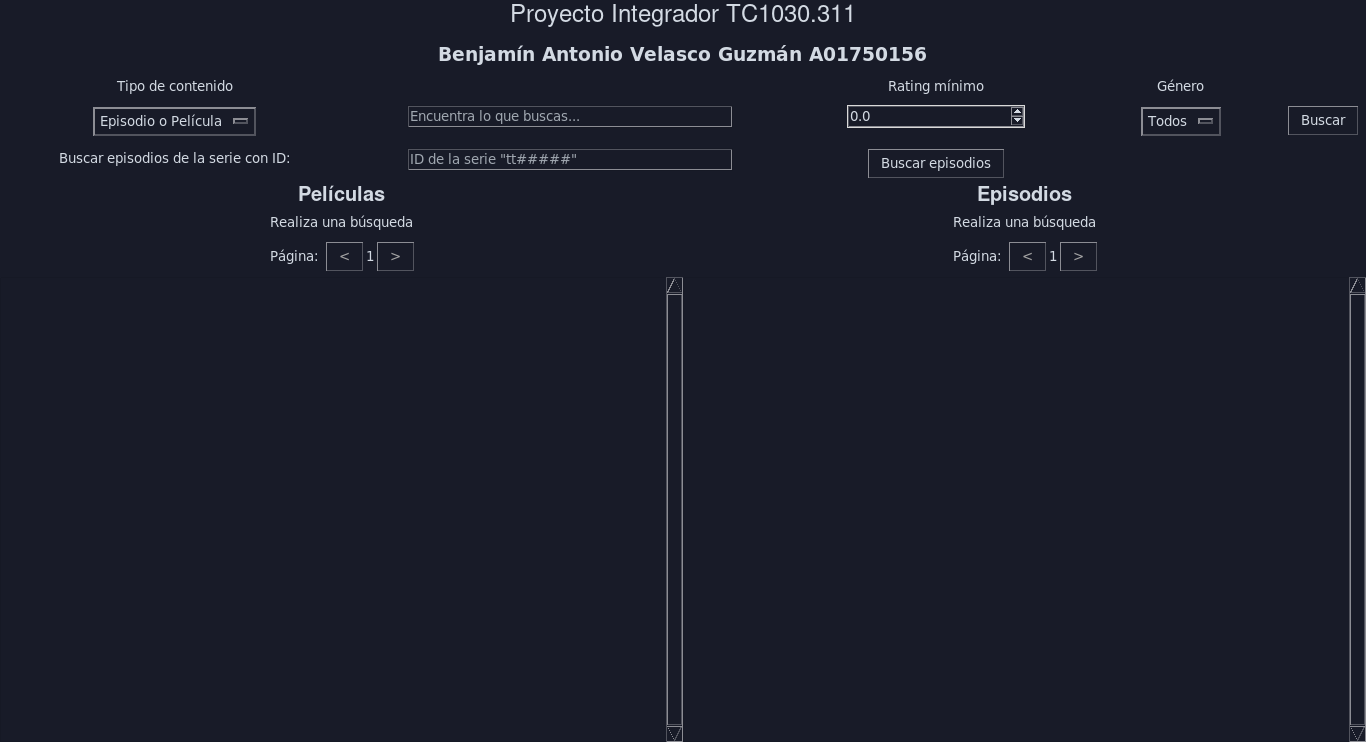
\includegraphics[width=0.9\linewidth]{interface-start}
	\caption{Presentación de la aplicación}
\end{figure}

Es importante aclarar que las imágenes a continuación muestran la información del episodio o película al lado de otra imagen, la cual fue colocada simplemente por fines estéticos y no representa nada, también fue colocada por términos de escalabilidad por si en determinado momento se llegara a requerir la imagen real del episodio, serie o película.

\subsection{Flujo básico}
A continuación se muestran imágenes de la ejecución de la aplicación y funcionamiento del flujo básico (cómo debería comportarse la aplicación si todos los datos ingresados son correctos)\newline

\begin{center}
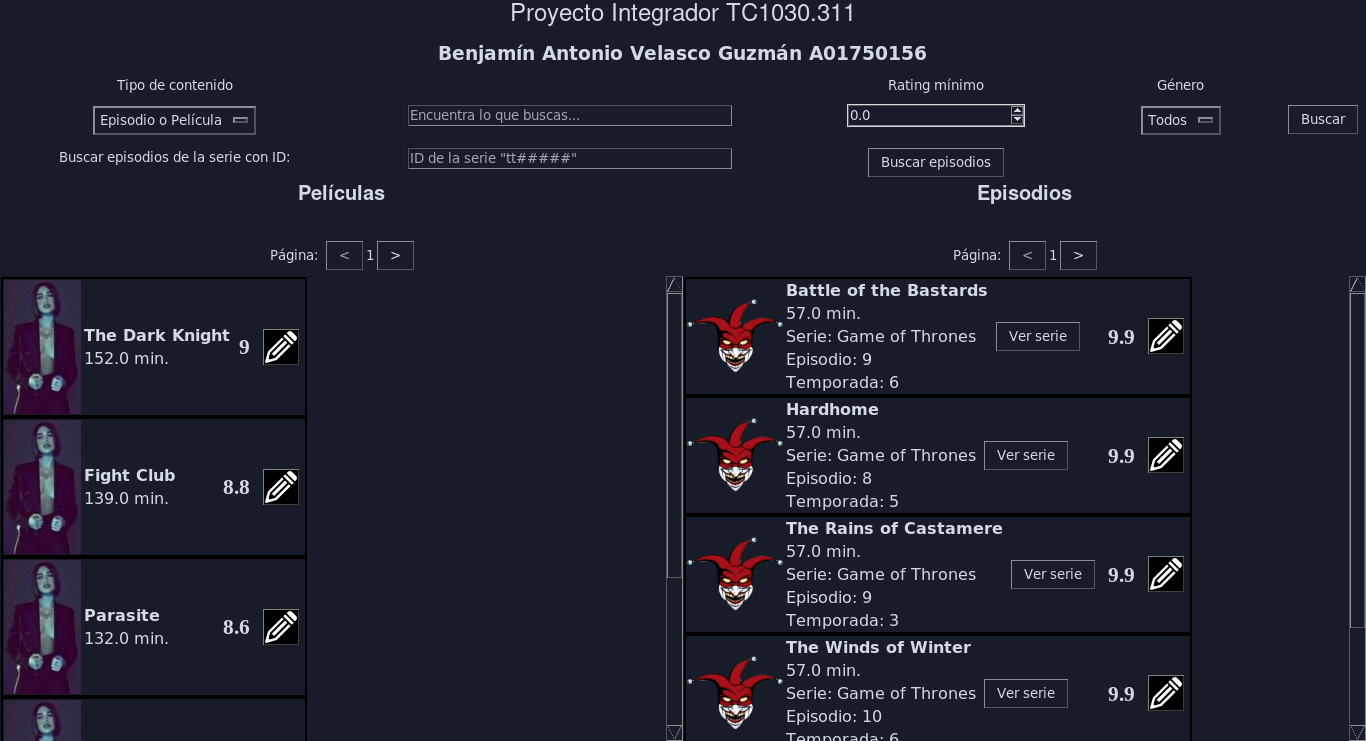
\includegraphics[width=0.9\linewidth]{interface-buscar}
\captionof{figure}{Búsqueda de cualquier película o episodio, con cualquier nombre, cualquier género y rating mínimo de 0}

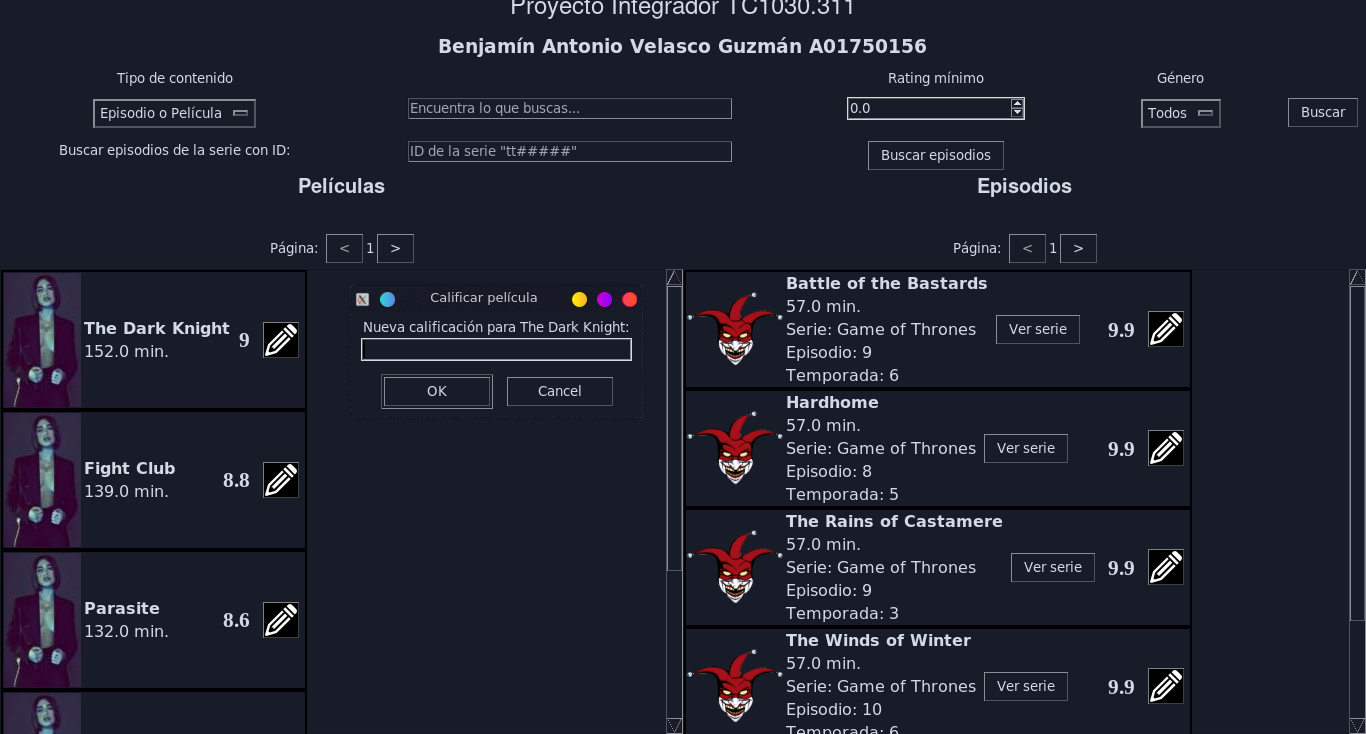
\includegraphics[width=0.9\linewidth]{interface-mod-movie}
\captionof{figure}{Cuadro de diálogo para modificar el rating de una película}

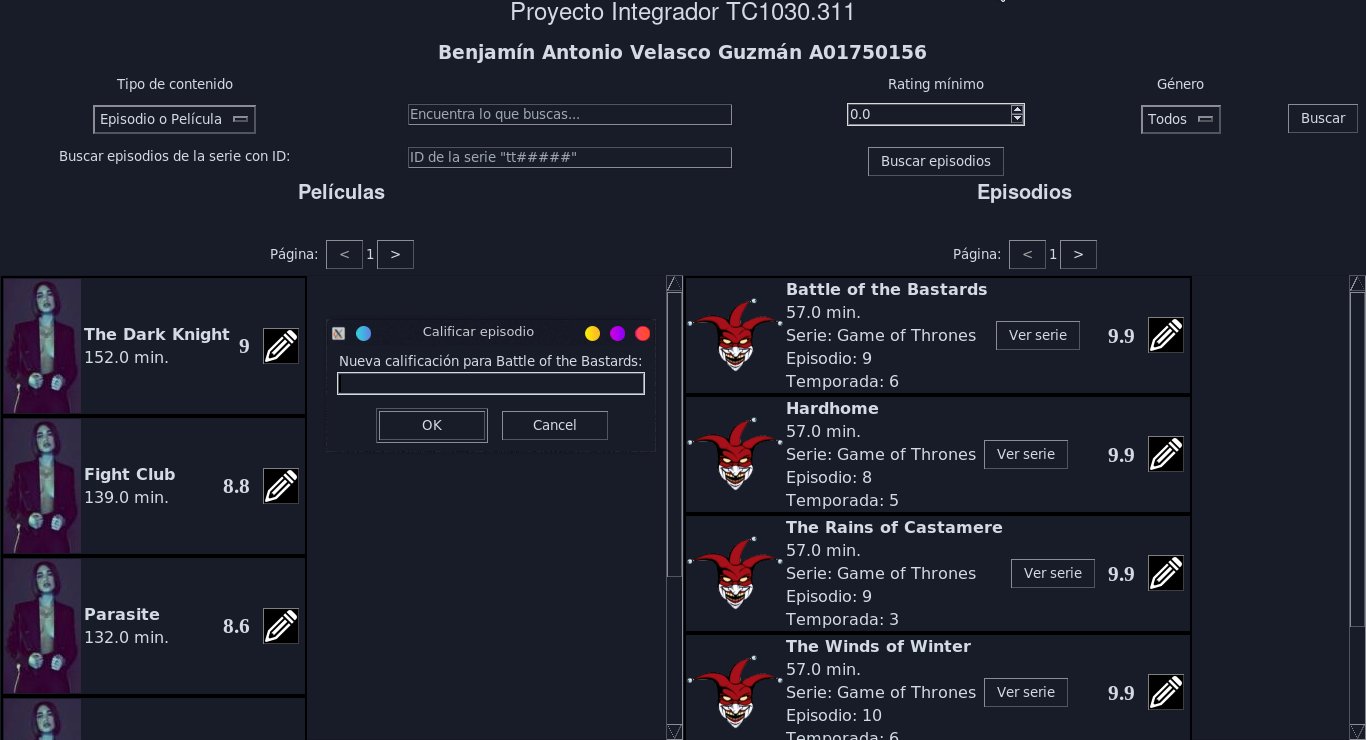
\includegraphics[width=0.9\linewidth]{interface-mod-episode}
\captionof{figure}{Cuadro de diálogo para modificar el rating de un episodio}

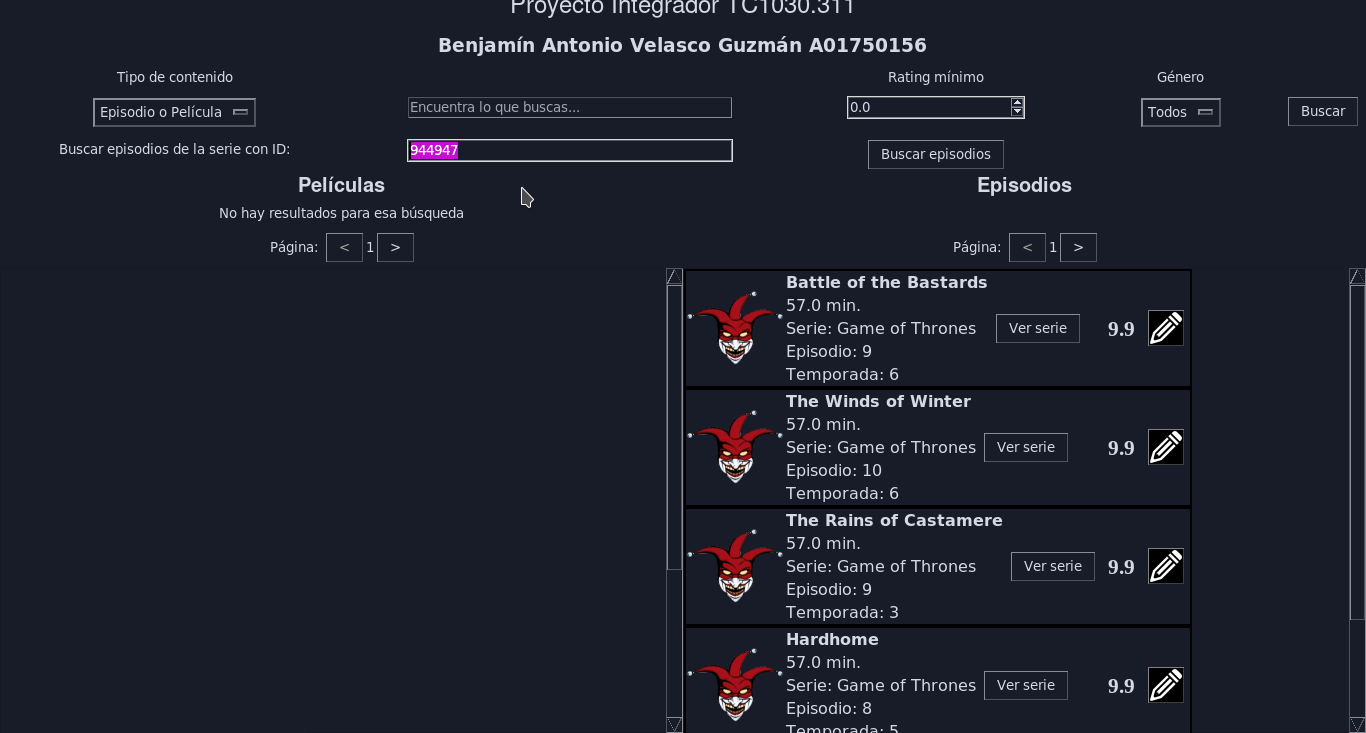
\includegraphics[width=0.9\linewidth]{interface-search-serie}
\captionof{figure}{Búsqueda de episodios de una serie}

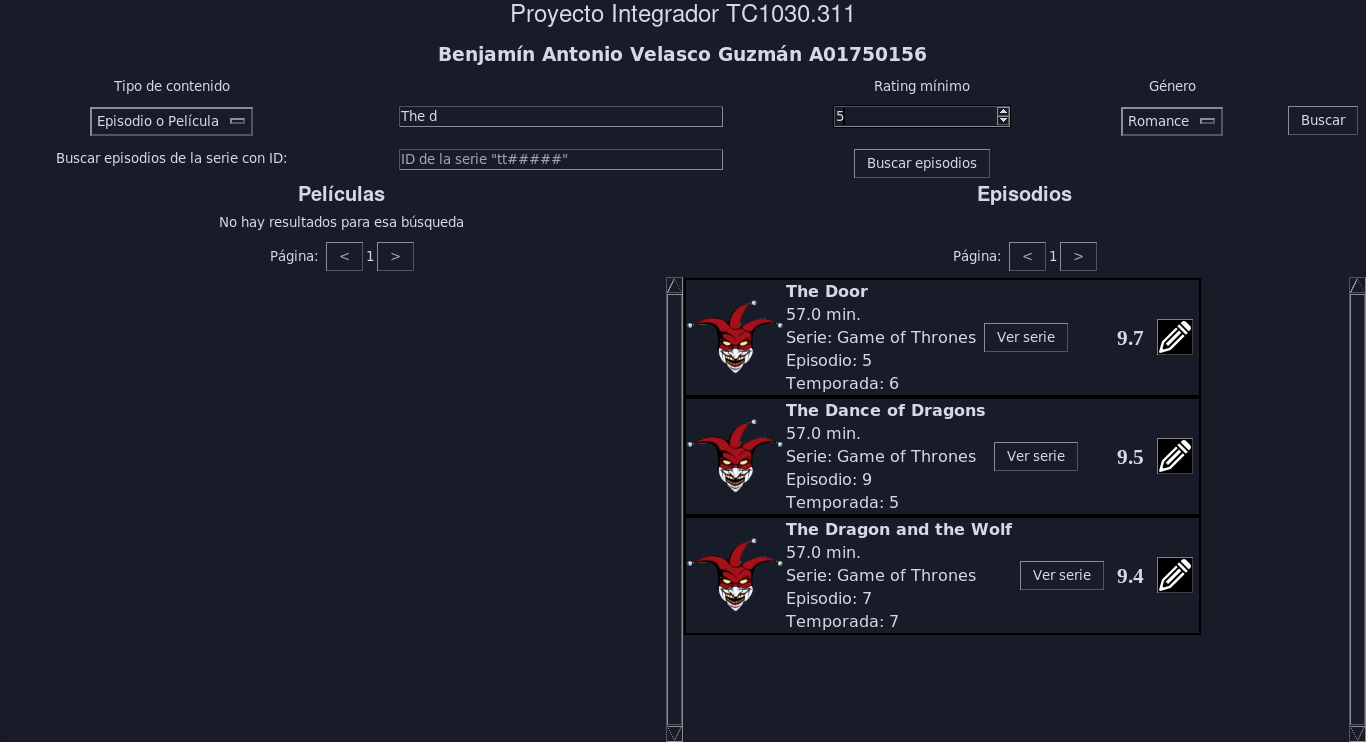
\includegraphics[width=0.9\linewidth]{interface-search-romance}
\captionof{figure}{Búsqueda de cualquier película o episodio, que empiece con los caracteres "The d", con rating mínimo de 5 y de género Romance}

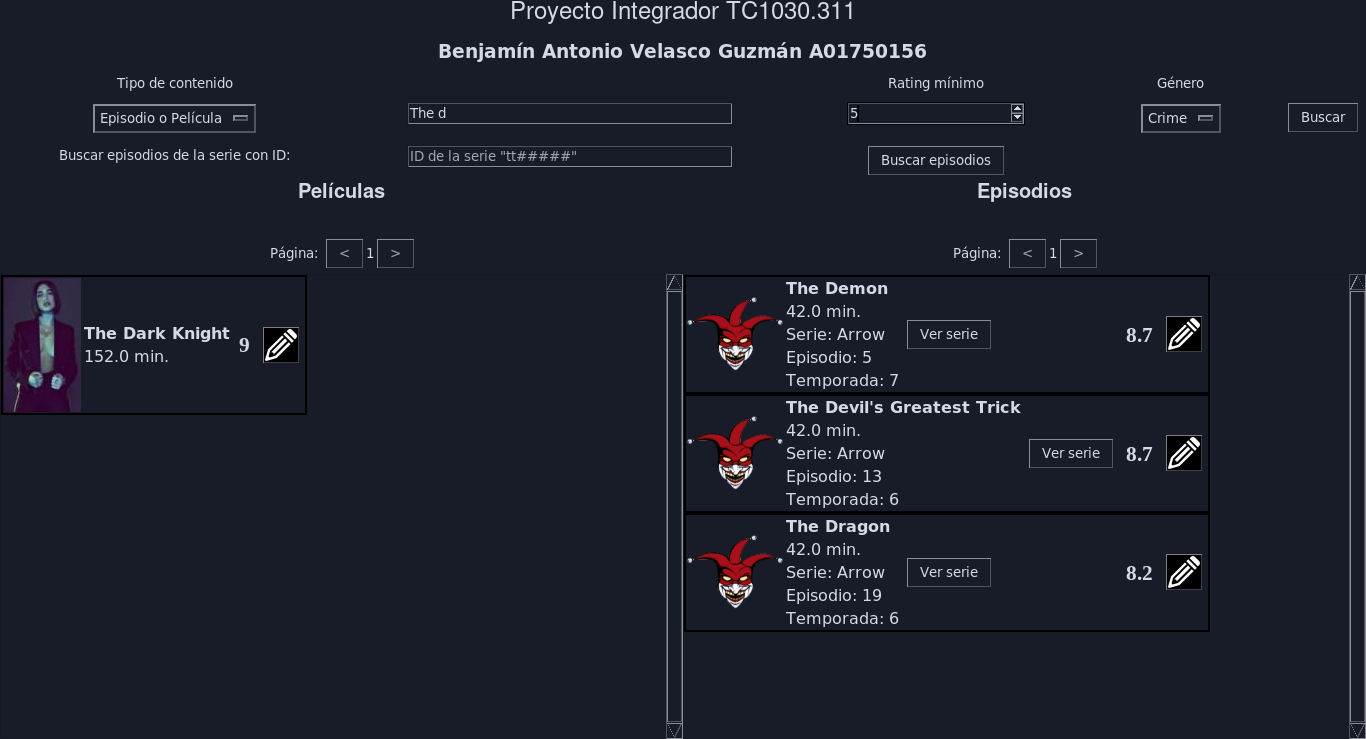
\includegraphics[width=0.9\linewidth]{interface-search-crime}
\captionof{figure}{Búsqueda de cualquier película o episodio, que empiece con los caracteres "The d", con rating mínimo de 5 y de género Crime}
\end{center}

Nótese la diferencia entre los valores de los parámetros de búsqueda y los resultados entre las dos últimas imágenes.

\subsection{Flujos de excepción}
A continuación se muestran imágenes de la ejecución de la aplicación y funcionamiento cuando existe algún flujo de excepción (cómo debería comportarse la aplicación si algún valor no es válido)

\begin{center}
	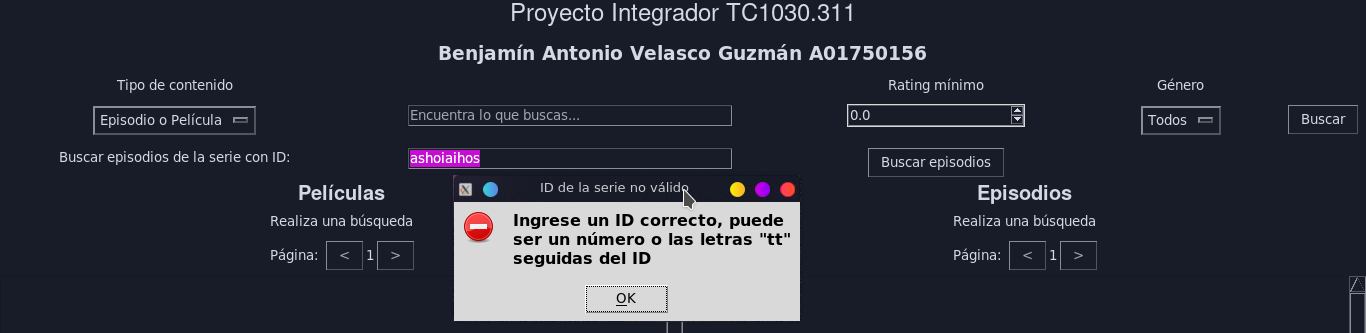
\includegraphics[width=0.9\linewidth]{interface-invalid-id}
	\captionof{figure}{Mensaje de error si al buscar una serie se ingresa un ID no válido}

	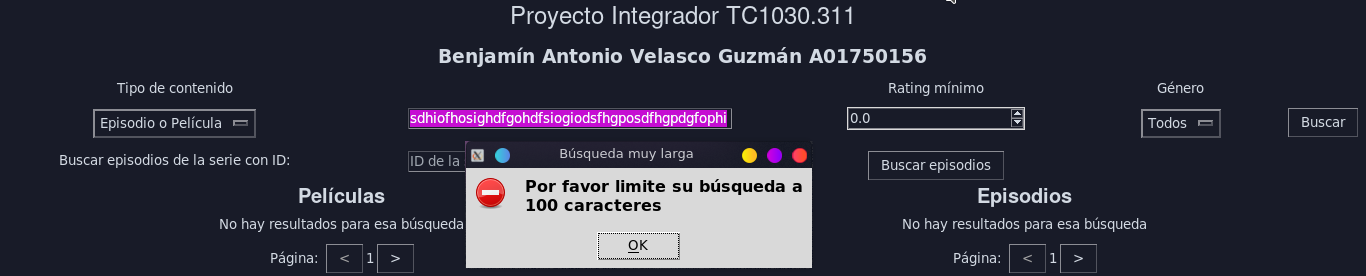
\includegraphics[width=0.9\linewidth]{interface-search-limit}
	\captionof{figure}{Mensaje de error si al buscar contenido por nombre se ingresan más de 100 caracteres}

	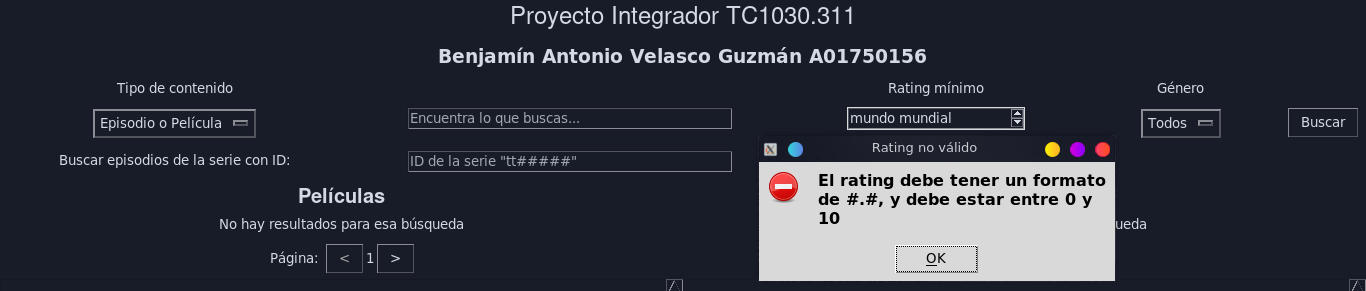
\includegraphics[width=0.9\linewidth]{interface-invalid-rating}
	\captionof{figure}{Mensaje de error si al buscar contenido por rating mínimo se ingresan valores que no sean números enteros o flotantes}

	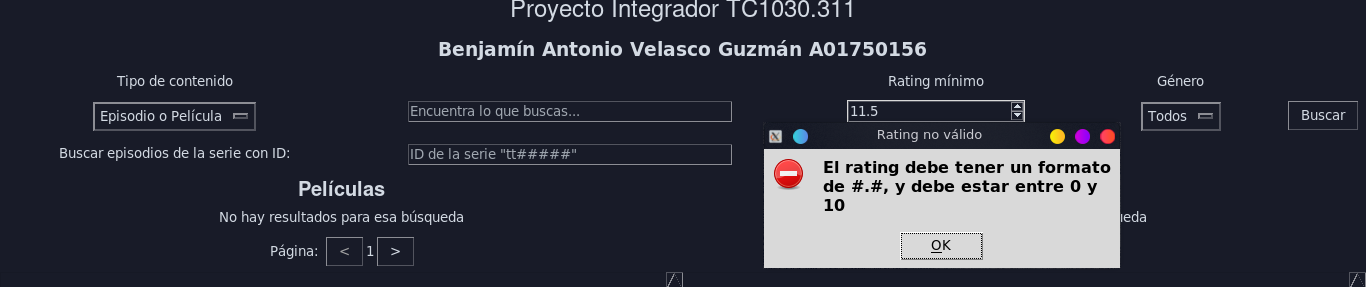
\includegraphics[width=0.9\linewidth]{interface-invalid-rating2}
	\captionof{figure}{Mensaje de error si al buscar contenido por rating mínimo se ingresan valores fuera de rango}
\end{center}